\chapter{Background}

\section{Reinforcement Learning}

Reinforcement Learning (RL) is a branch of machine learning, alongside supervised learning and unsupervised learning, that defines a set of algorithms meant to learn how to act in a specific environment without the need of labeled data to learn from. 

The algorithm defines the agent that learns a given task, for example, walking, driving and playing a game, by trial and error, while interacting with an environment which can be real or simulated. Whenever the agent makes a set of good actions it receives a positive reward, which makes such actions more likely in the future. State, action and reward are the most important concepts in RL. The state represents the current situation of the environment. If the agent is a humanoid robot and the task is walking, one possible state representation is the positions of its actuated joints. The action set or space in case of continuous domain, describes what the agent can do in a particular state. In the humanoid robot example above, the action space is a n-dimensional vector where each dimension represents the torque command to each of the n joint motors. Finally the reward is a measure of how good are the actions carried out by the agent. 

\begin{wrapfigure}{r}{0.6\textwidth}
  \begin{center}
    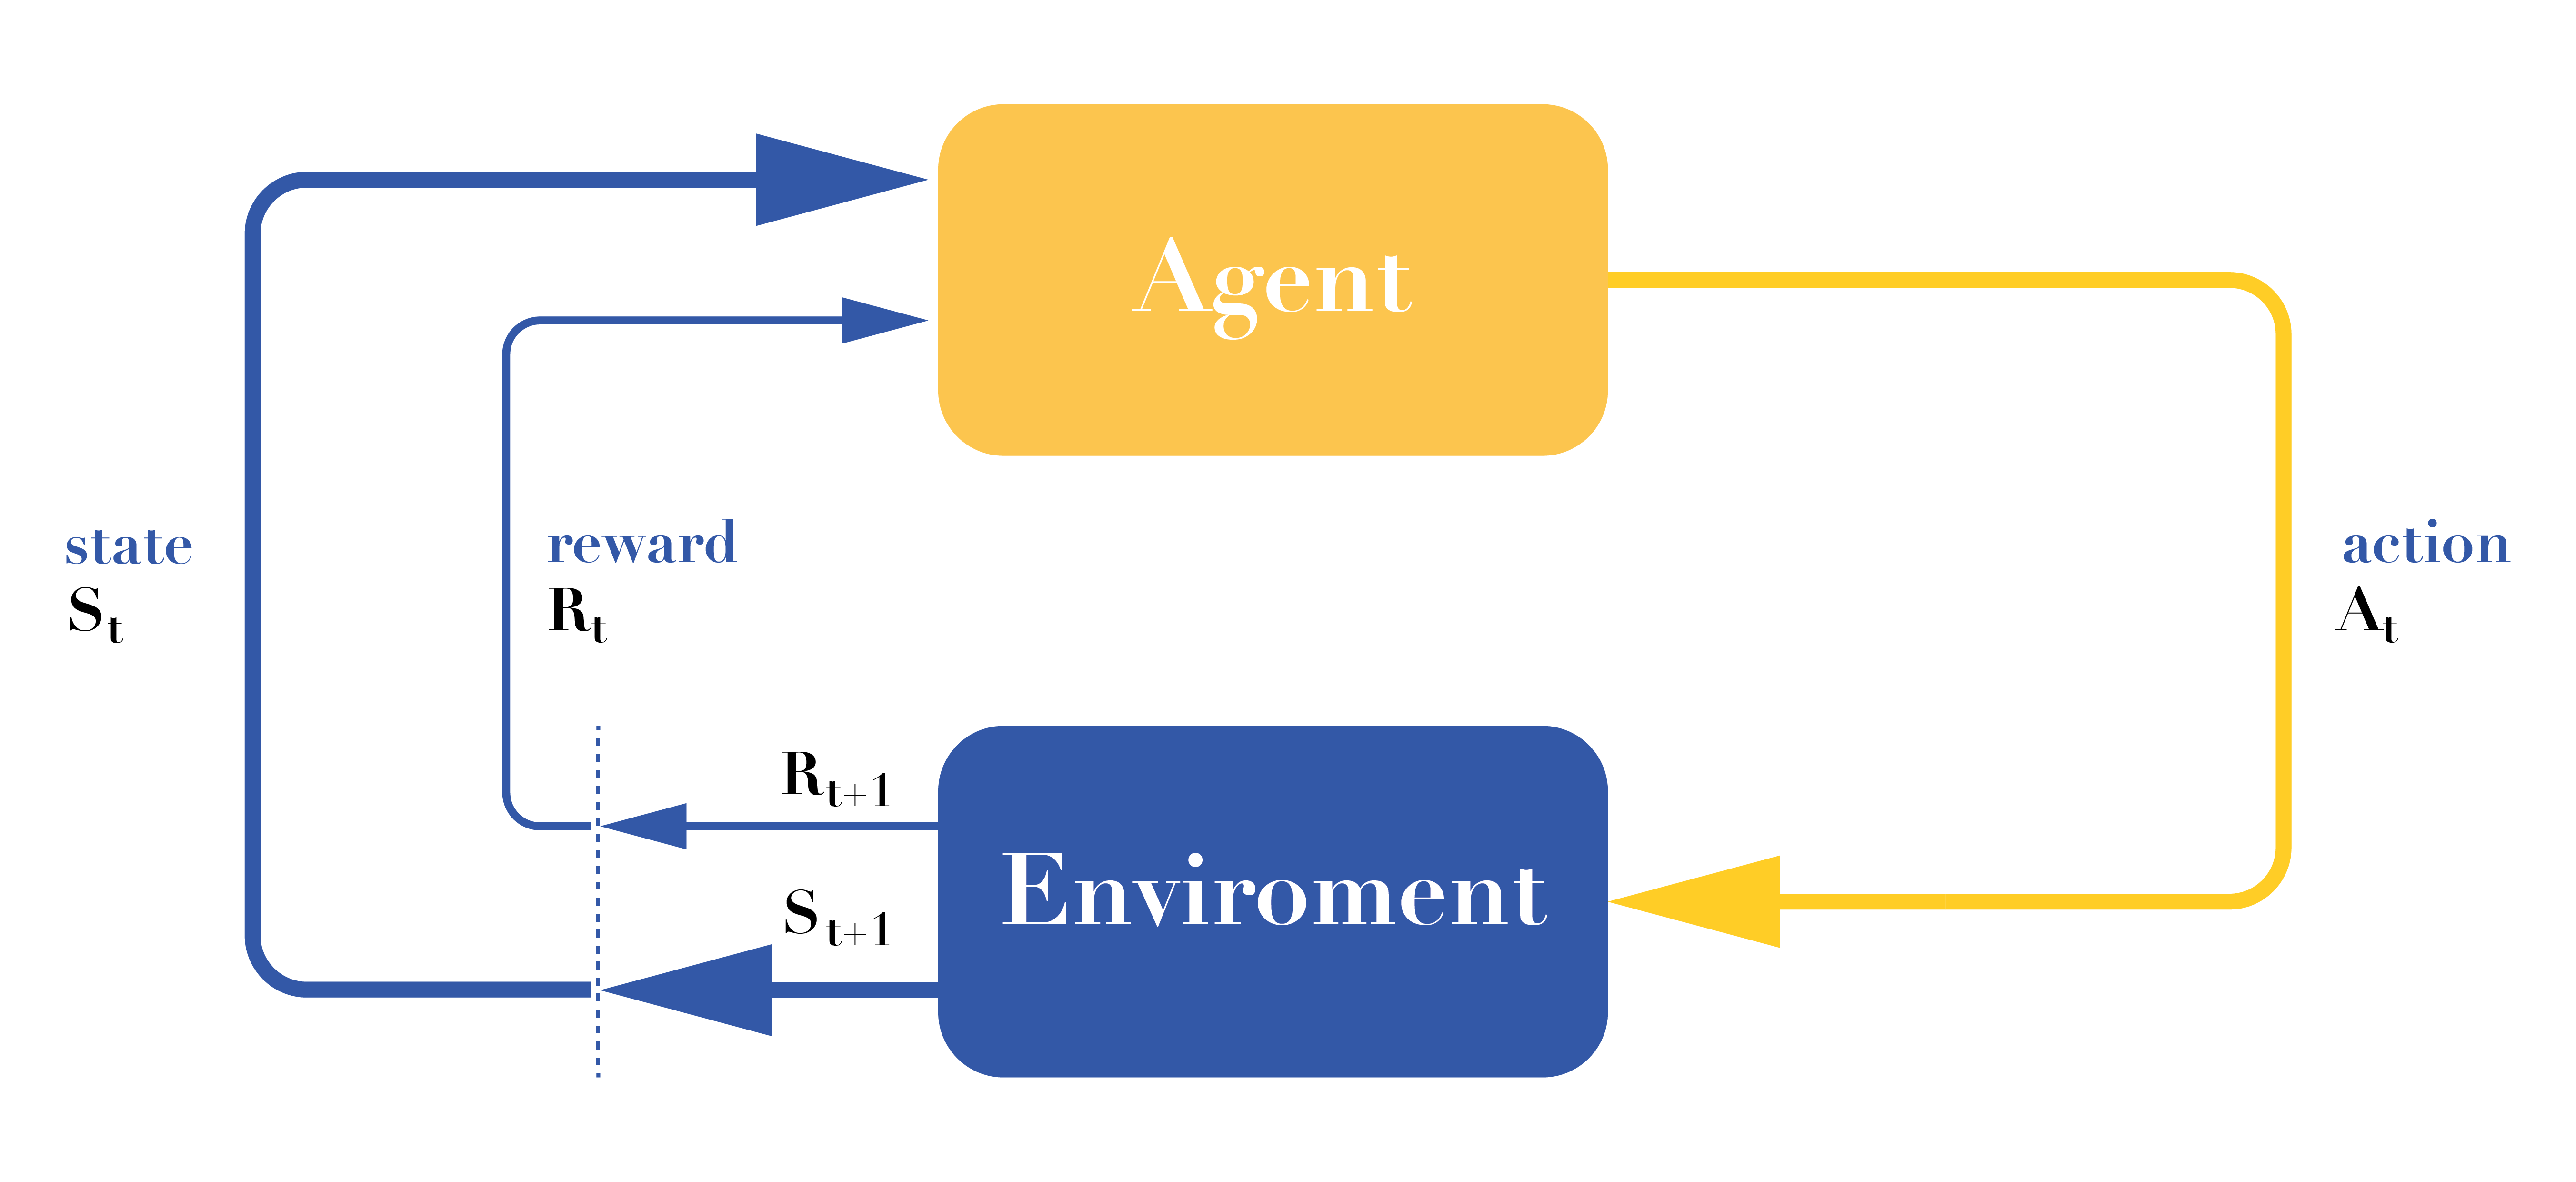
\includegraphics[width=0.6\textwidth]{background/rl.png}
  \end{center}
  \caption{Basic reinforcement learning}
  \label{fig:rl}
\end{wrapfigure}

The reward function, usually human-designed, assigns a score to the action taken by the agent. Every action that leads to a \textit{good} state increases the score and vice-versa. As described in Figure \ref{fig:rl} the agent interacts with the environment in discrete time steps. At time $t$ it gets the current state $s_{t}$ and the associated reward $r_{t}$ then the action $a_{t}$ is chosen from the set of available actions. After receiving the chosen action, the environment moves to a new state $s_{t+1}$ and the reward $r_{t+1}$ is given back to the agent. The total discounted reward (also known as return) to be maximized is:

\begin{equation}
  \label{eq:totalreward}
  R=\sum _{t=0}^{T}\gamma ^{t}r_{t}
\end{equation}
where $T$ is the time horizon (eventually $\infty$), $\gamma \in [0,1)$ is the discount factor which makes future rewards worth less than immediate rewards. The reward function is fundamental to the agent in order to learn and optimize a policy function $\pi$:
\begin{align}
  \displaystyle \pi &:A\times S\rightarrow [0,1] &  \displaystyle \pi (a,s)&=\Pr(a_{t}=a\mid s_{t}=s) \label{eq:label1}
\end{align}
The policy is a mapping that gives the probability of taking action $a$ in state $s$. By following the policy the agent takes the action that maximizes the reward. However, the policy, especially during training, is not deterministic. This is due to one of the fundamental challenges in RL, i.e. the exploration-exploitation dilemma \citep{Sutton1998}. Indeed, the agent needs to repeat the actions it already knows to be rewarding but, at the same time, it needs to explore the environment to discover actions that can lead to an even higher reward. 
The final goal of the algorithm is to learn a policy that maximizes the expected cumulative reward:
\begin{equation}
  \label{eq:rlobj}
  J(\pi)=\mathbb{E}_{\pi}[\sum _{t=0}^{T}\gamma ^{t}r(s_{t},a_{t})]
\end{equation}
The expectation term is added because both the policy and the environments are usually stochastic.
There are multiple ways to learn the optimal policy $\pi^{*}(s)$ assuming the \textit{State Transition probability matrix} $P$ that describes the probability of moving from one state to any successor state is known. The first one is called \textit{Value iteration}, which exploits the state value function $V^{\pi}(s)$ and the action value function $Q^{\pi}(s, a)$. The state value function $V$ is the expected return starting from the state s and following the policy $\pi$:

\begin{equation}
  \label{eq:statevalue}
  V(s) = E_{\pi}[\sum_{t=0}^{T-1} \gamma^t r_t \mid s_t=s]
\end{equation}
while the action value function $Q$ is the expected return starting from the state s and taking action $a$ by following the policy $\pi$ :

\begin{equation}
  \label{eq:actionstatevalue}
  Q(s,a) = E_{\pi}[\sum_{t=0}^{T-1} \gamma^t r_t \mid s_t=s, a_t = a]
\end{equation}
There is an important relationship between the two functions \ref{eq:statevalue} and \ref{eq:actionstatevalue}, in fact they can be written in terms of each other:

\begin{equation}
  \label{eq:statevaluefromQ}
  V(s) = \sum_{a\in A} \pi(a \mid s) Q^{\pi} (s,a)
\end{equation}

\begin{equation}
  \label{eq:actionstatevaluefromV}
  Q(s,a) = \sum_{s'\in S} P(s' \mid s,a) [r(s,a,s') + \gamma V (s')].
\end{equation}
where $P$ is the state transition matrix that gives the probability of reaching the next state $s\textit{'}$ given the state $s$ and action $a$ and $r$ is the reward function that returns the reward value associated with transitioning to the next state $s'$ by taking the action $a$ in state $s$.

In \textit{Value Iteration}, the value function $V$ is randomly initialized and the algorithm, illustrated in Listing \ref{lst:valueiteration}, repeatedly updates the values of $Q$ and $V$ for each state until convergence. When value iteration terminates the functions $Q$ and $V$ are guaranteed to optimal.

\begin{center}
  \begin{minipage}{0.65\linewidth}
    \lstinputlisting[escapeinside={(*}{*)}, caption=Value iteration pseudo code from \citet{Alpaydin:2014:IML:2635955}, captionpos=b, label=lst:valueiteration]{valueiteration.pseudo}
    \end{minipage}
\end{center}
Finally the optimal policy $\pi^{*}$ can be inferred from the optimal $Q^{*}$ function with:
\begin{equation}
  \label{eq:pifromq}
  \pi^{*}(s) = argmax_a Q^{*}(s,a)
\end{equation}
The optimal policy aims at choosing the actions that maximize the optimal $Q$ function all states.

Since the fundamental quantity for the agent is the policy, another way of training the agent is to learn a policy without extracting it from the action-value function $Q$. Therefore, the so-called \textit{Policy Iteration} algorithm seeks to learn the policy directly by updating it at each step as shown in Listing \ref{lst:policyiteration}
\begin{center}
  \begin{minipage}{0.65\linewidth}
    \lstinputlisting[escapeinside={(*}{*)}, caption=Policy iteration pseudo code from \citet{Alpaydin:2014:IML:2635955}, captionpos=b, label=lst:policyiteration]{policyiteration.pseudo}
    \end{minipage}
\end{center}
Policy iteration is also guaranteed to converge to the optimal policy and it often takes less iterations to converge than the value iteration algorithm.

A major problem arises when the \textit{the State Transition Matrix} of the environment is not known to the agent or the number of possible states is too big to be stored in tables, as for example when the state is an image and/or the action space is continuous. Deep RL algorithms use Deep Neural Networks in order to approximate $Q$ and $V$ instead of storing them in tables. Indeed, DNNs can represent states and actions in a compact way thanks to their ability to generalize to unseen data. 

Besides the quantity that needs to be learnt, i.e. the value functions or the policy, RL algorithms are also categorized by the way such quantities are updated. On-Policy methods evaluate and improve the same policy which is being used to select actions. Off-Policy methods can optimize a certain quantity (usually an action value function $Q$) with data coming from any policy. Such methods are typically more efficient than on-policy methods, as they can reuse already collected experience multiple times. In order to reuse previously gathered data, off-policy methods randomly sample training data from the past experience stored in buffers, generally called replay buffer. The replay buffer contains a collection of experience tuples ($s$, $a$, $r$, $s'$), where $s$ is the state, $a$ the action taken in state $s$, $r$ the corresponding scalar reward and $s'$ the new state reached by taking action $a$.

\section{OpenAI Gym interface}

Gym is an open source library that defines a standard API to handle training and testing of RL agents, while providing a diverse collection of simulated environments. The environment is of primary importance to a RL algorithm since it defines the world the agent lives and operates in. 

\begin{wrapfigure}{r}{0.6\textwidth}
  \begin{center}
    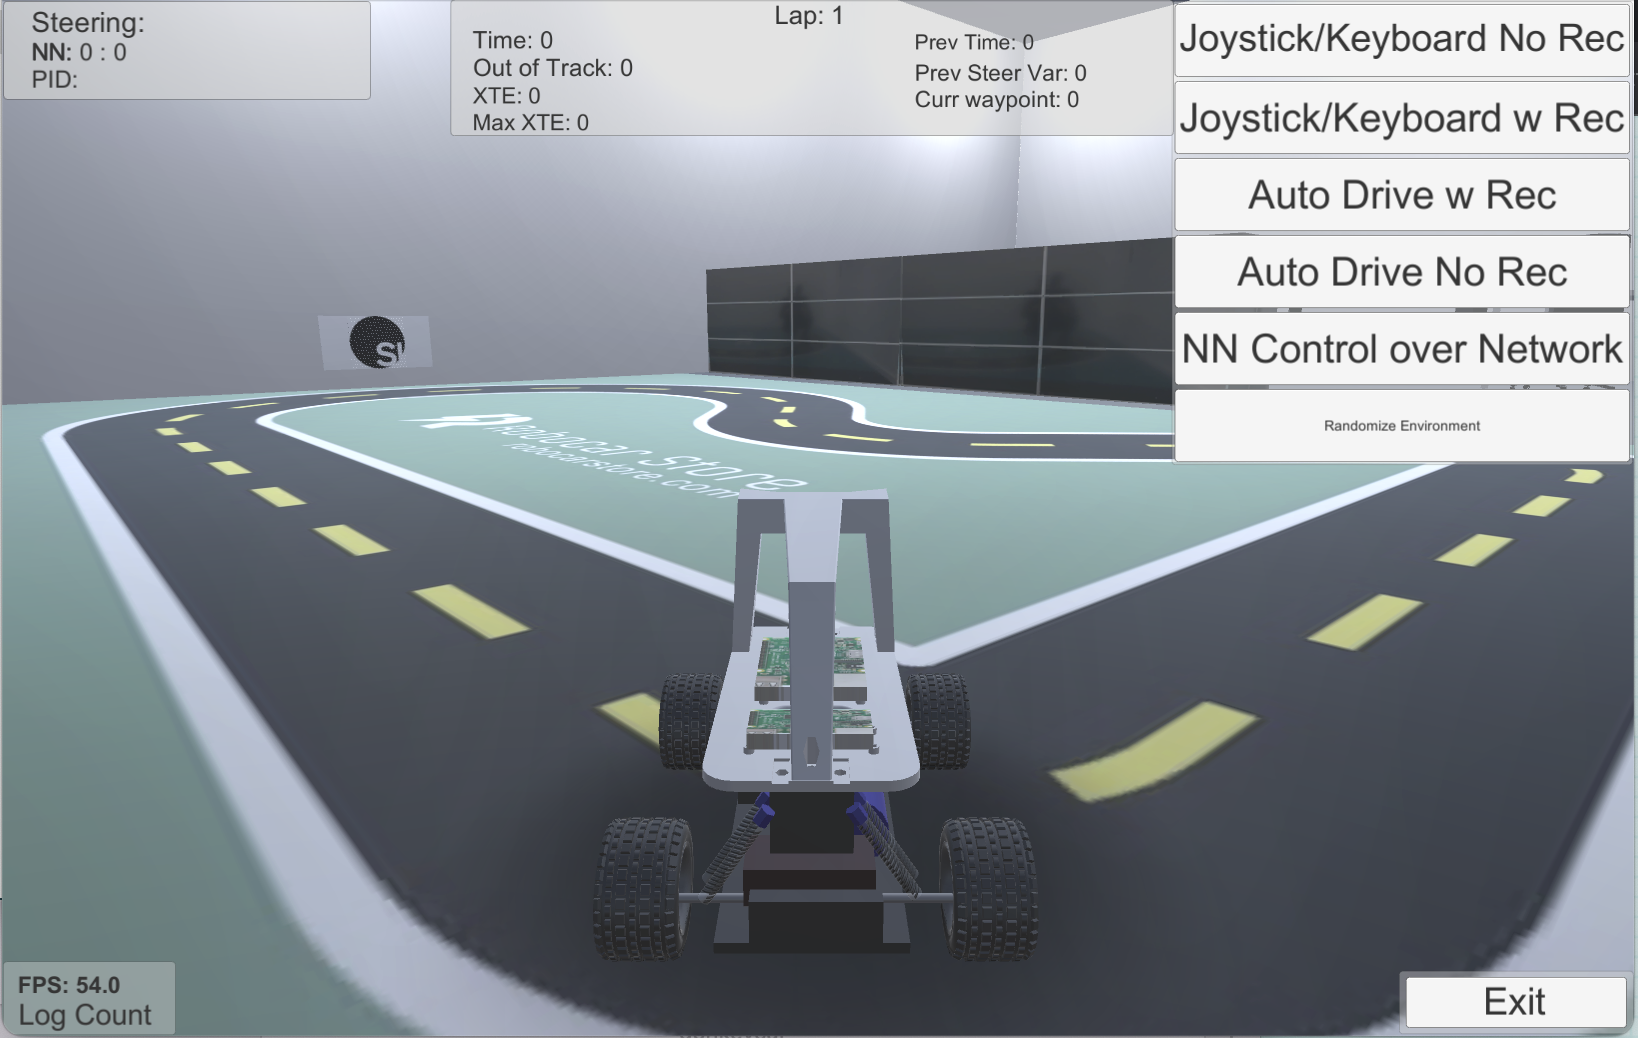
\includegraphics[width=0.6\textwidth]{background/env.png}
  \end{center}
  \caption{DonkeyCar environment}
  \label{fig:gym}
\end{wrapfigure}

The standard interface designed by Gym, makes it easy to interact with environments, both made available by Gym and externally developed. The Gym interface is simple and capable of representing general RL problems. The DonkeyCar environment, shown in Figure \ref{fig:gym} and used in this thesis, is an example of custom environment. With Gym we can define the \textit{ action space} of the car, i.e., all the operations the agent controlling the car can carry out, such as steer and accelerate. Furthermore, we can also define the \textit{observation space}, i.e., what the agent perceives about the environment at each timestep. For instance, a possible observation space for an agent controlling a car is the camera image.

Moreover, the Gym documentation provides a reference template, shown in Listing \ref{lst:gym}, that describes what are the fundamental methods a Gym environment should implement to work properly.
Any existing environment built with Gym implements the following methods:

\begin{center}
  \begin{minipage}{0.45\linewidth}
    \lstinputlisting[caption="Gym template", captionpos=b,  label=lst:gym]{gym.py}
    \end{minipage}
\end{center}

\begin{itemize}
  \item \textbf{init:} every environment should extend the gym.Env class and override the variables \textit{observation\_space} and \textit{action\_space} specifying the type of observations and actions. According to the Gym notation the state of the environment is called \textit{observation} since, in general, the state is not fully observable. Therefore, the observation is the observable part of the state, i.e. what the agent can perceive with its sensors;
  \item \textbf{step:} this method is the primary interface between environment and agent. It takes as input the action to be carried out in the environment and returns a tuple (observation, reward, done) containing the next observation resulting from the action executed in the environment, the corresponding reward value and a boolean flag signaling the end of the \textit{episode}. Indeed, a Gym environment models episodic RL tasks, i.e. finite tasks that terminate when certain conditions hold;
  \item \textbf{reset:} this method resets the environment to its initial conditions returning the initial observation. This method is called to initialize the environment and at the end of each episode, such that the agent starts each episode always with the same initial conditions;
  \item \textbf{render:} this method renders the environment when a parameter \textit{mode='human'} is passed.
  \item \textbf{close:} this method performs any necessary cleanup before closing the environment.
\end{itemize}

Beside the API interface, Gym provides a set of wrappers to modify an existing environment without having to change its underlying code directly. The three main things a wrapper does are:

\begin{itemize}
  \item Transform actions before they are executed in the underlying environment (e.g., ActionWrapper);
  \item Transform observations that are returned by the underlying environment (e.g., ObservationWrapper)
  \item Transform rewards that are returned by the underlying environment (e.g., RewardWrapper)
\end{itemize}

 Furthermore, custom wrappers can be implemented by inheriting from the \textit{Wrapper} class.

\section{Soft Actor Critic - SAC}
The soft actor critic algorithm \citep{art:sac} is a state-of-the-art RL algorithm designed to outperform prior on-policy and off-policy methods in a range of continuous control benchmark tasks. 

It aims to both increase the \textit{sample efficiency} and the robustness of the policy at test time. A poor sample efficiency is typical of on-policy RL methods since they require new sample to be collected for each gradient step. In order to improve the sample efficiency, SAC adopts an off-policy approach where the experience is stored in a replay buffer such that it can be reused multiple times during training. Moreover, SAC is based on the maximum entropy framework which maximizes both the expected return and the entropy of the policy. This objective is expressed in the following equation:

\begin{equation}
  J(\pi)=\mathbb{E}_{\pi}[\sum _{t=0}^{T}\gamma ^{t}r(s_{t},a_{t})+\alpha H(\pi(\cdot \mid s_{t}))]
\end{equation}

where $\alpha$ is a temperature parameter that weighs the entropy term and thus controls the policy stochasticity. Maximizing both the expected reward and the entropy of the policy is beneficial to obtain policies that are robust w.r.t. unexpected situations at testing time. Moreover, training a stochastic policy encourages a wide exploration of the environment, promoting diverse behaviors of the agent.

\section{Generative Adversarial Networks - GAN}

\begin{wrapfigure}{r}{0.6\textwidth}
  \begin{center}
    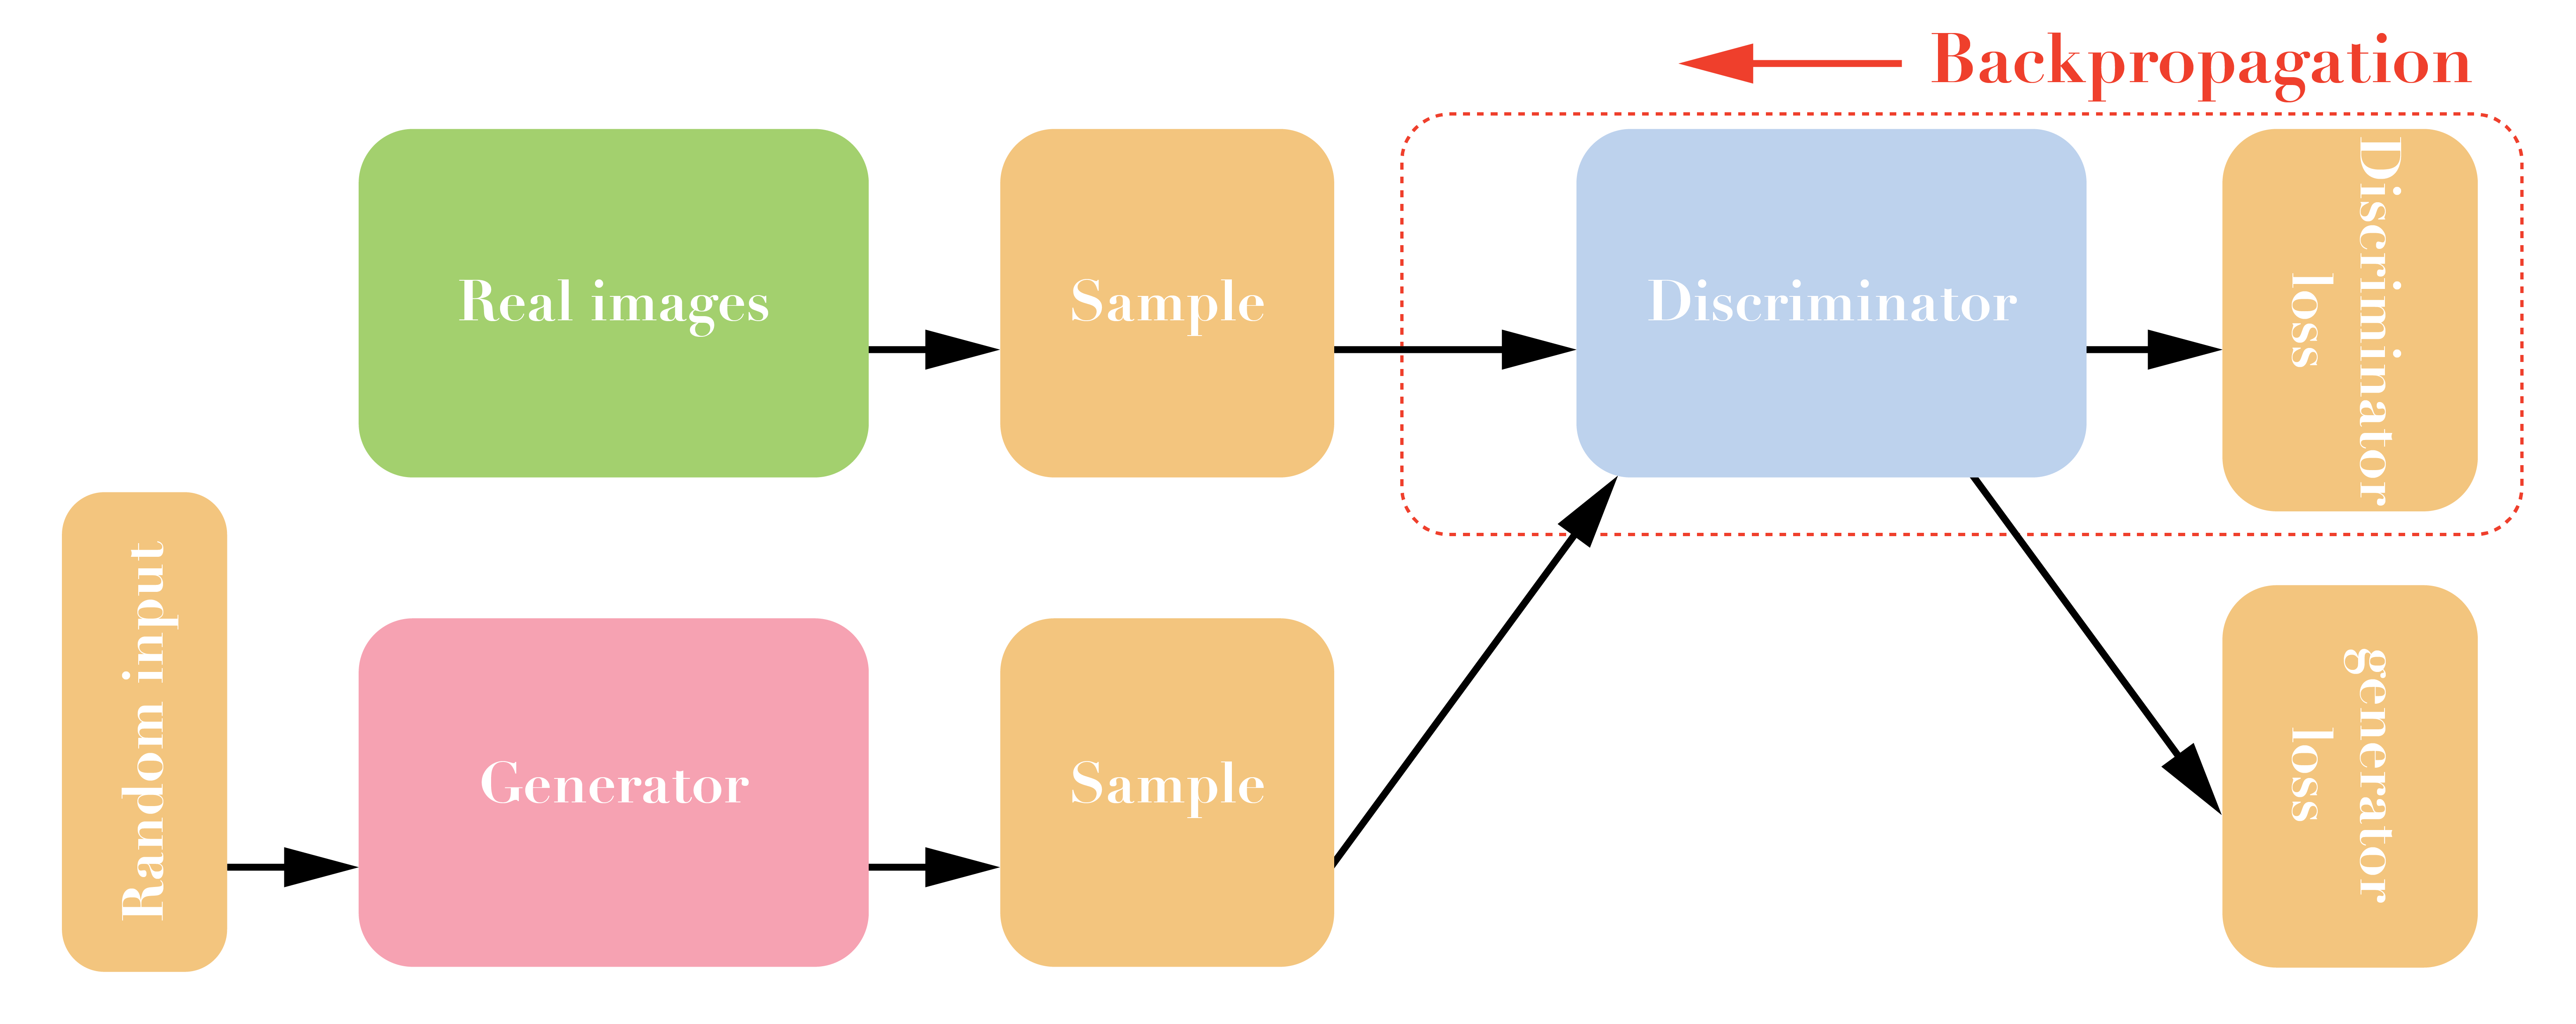
\includegraphics[width=0.6\textwidth]{background/gan.png}
  \end{center}
  \caption{GAN diagram}
  \label{fig:gan}
\end{wrapfigure}

Generative Adversarial Network is a framework introduced by \citet{art:gan} for training generative models in an unsupervised fashion. GANs can be used, for example, to generate visual paragraph \citep{Liang_2017_ICCV}, realistic text \citep{pmlr-v70-zhang17b}, photographs of human faces \citep{https://doi.org/10.48550/arxiv.1710.10196} and Image-to-Image translation \citep{Isola_2017_CVPR}.
The learning process involves two neural networks that are trained in an adversarial way, i.e. with a contrasting objective. Indeed, as shown in Figure \ref{fig:gan}, the generator G generates inputs (e.g., images) starting from random noise and the discriminator D needs to distinguish whether such inputs belong to the original dataset or not. GANs fall under the branch of unsupervised learning since the training process does not need labeled data as the generator is guided by the discriminator in order to generate inputs that resemble those of the training dataset. The discriminator $D$ is trained to maximize the probability of returning the correct label when given both training examples and examples generated by the generator $G$. At the same time the objective of generator $G$ is to minimize the following loss function:

\begin{equation}
  \label{eq:gloss}
  L_G =log(1-D(G(z)))
\end{equation}

where $z$ is the random noise vector, i.e., the latent vector, $D(G(z))$ is the probability that the generated example $G(z)$ comes from the training dataset (represented by the distribution $p_{x}$ where X is the training dataset and $p_{x}$ represents all the possible images that can be in X), which means that $1-D(G(z))$ is the probability that $G(z)$ does not come from from $p_{x}$. Indeed, the objective of the generator $G$ is to generate examples that are indistinguishable from the training examples for the discriminator $D$.

In particular, in order to learn the generator's distribution $p_{g}$ over the training dataset $X$ such that $p_{g}\approx p_{x}$, the authors define a distribution over latent vectors $p_{z}(z)$, which is mapped into the data space with the generator $G(z, \theta_{g})$. Moreover, the discriminator $D(x;\theta_{d})$, with $x \sim p_{g}$, outputs a single value which estimates the probability of $x$ coming from the distribution $p_{x}$ rather than $p_{g}$. $D$ and $G$ are both differentiable functions represented by a neural network with parameters $\theta_{d}$ and $\theta_{g}$ respectively.

In other words, the discriminator and the generator play a minimax game to optimize the function $V(G,D)$:
\begin{equation}
  \label{eq:ganloss}
  min_G max_D V(G,D) = \mathbb{E}_{x\sim \rho_{data}(x)}[log D(x)] + \mathbb{E}_{z\sim \rho_{z}(z)}[log (1-D(G(z)))]
\end{equation}

\section{CycleGAN}
Image-To-Image translation is a complex task where the goal is to transform an image from one domain to another and vice-versa, as shown in Figure \ref{fig:translation}.

\begin{wrapfigure}{r}{0.5\textwidth}
  \begin{center}
    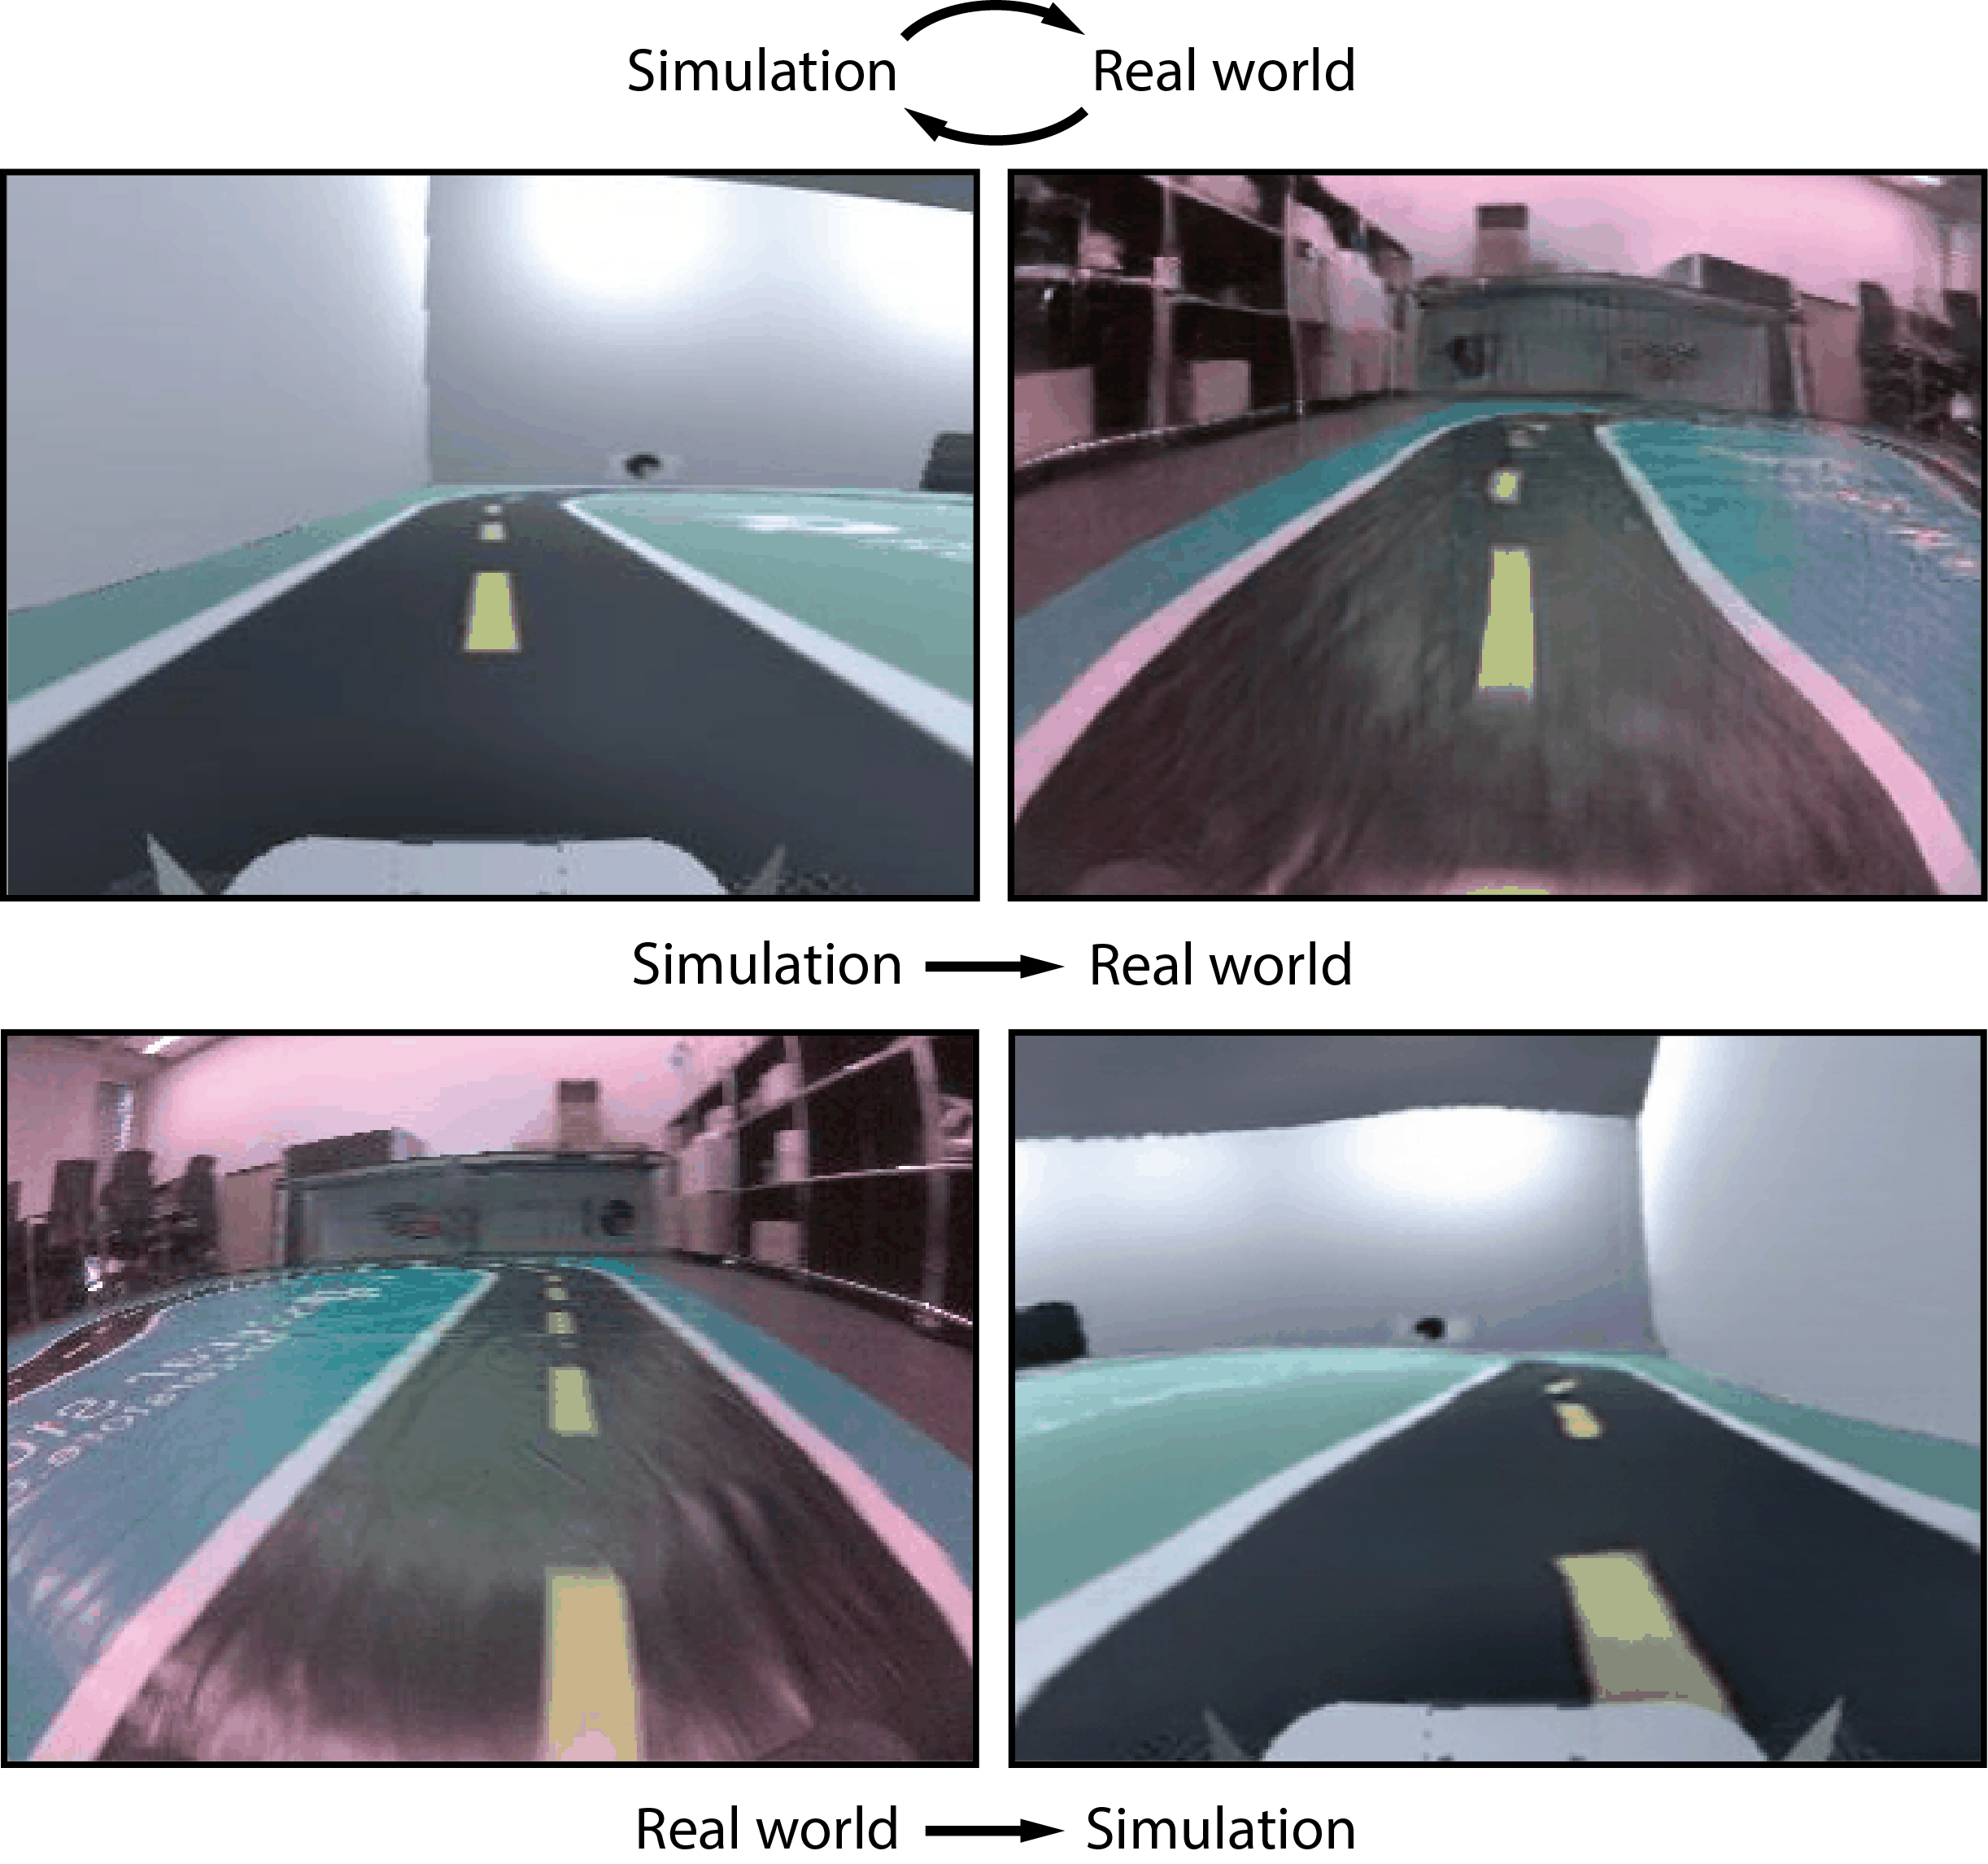
\includegraphics[width=0.5\textwidth]{background/imagetranslation.png}
  \end{center}
  \caption{Image-to-image translation example \citep{CycleGAN2017}. \matteo{Replace figure with Donkey sim2real}}
  \label{fig:translation}
\end{wrapfigure}

Prior papers have been proposed to translate images from one domain to another, however they often require paired training examples between the domains [\citet{https://doi.org/10.48550/arxiv.1612.00835}, \citet{karakan}].
Such paired datasets can be very expensive or even impossible to gather, as in the case of object transfiguration ($horse \leftrightharpoons zebra$).

Cycle-Consistent Adversarial Networks from \citet{CycleGAN2017} (CycleGAN), aims to solve this problem in an unsupervised fashion. The main goal is to learn, using an adversarial loss, a mapping $G:X\rightarrow Y$, where $X$ and $Y$ are two sets representing different domains, such that the image $G(x) $ with $x\in X$ is indistinguishable from an image $y\in Y$. Since the mapping is highly under-constrained, an inverse mapping $F:Y \rightarrow X$ is introduced, together with a cycle-consistency loss to enforce $F(G(x)) \approx x$ and vice-versa.
To accomplish the goal two discriminators $D_{X}$ and $D_{Y}$ are provided. $D_{X}$ tries to distinguish between examples coming from one domain (i.e. represented by the distribution $p_{x}$) and their translations $F(Y)$ and vice-versa for $D_{Y}$. 
The full objective \ref{eq:cycleganloss} includes the adversarial losses and the cycle-consistency loss to encourage a consistent translation from one domain to the other:

\begin{equation}
  \label{eq:cycleganloss}
  L(G,F,D_{X}, D_{Y}) = L_{GAN}(G, D_{Y},X,Y) + L_{GAN}(F, D_{X},Y,X) + \lambda L_{cyc}(G,F)
\end{equation}

where the loss $L_{GAN}(G, D_{Y},X,Y)$ and $L_{GAN}(F, D_{X},Y,X)$ can be constructed from Equation in \ref{eq:ganloss}
% where the loss $L_{GAN}(G, D_{Y},X,Y)$ is described below and $L_{GAN}(F, D_{X},Y,X)$ can be derived similarly:
% \begin{equation}
% L_{GAN}(G, D_{Y},X,Y) = \mathbb{E}_{y\sim \rho_{data}(y)}[log D_{Y}(y)] + \mathbb{E}_{x\sim \rho_{data}(x)}[log (1-D_{Y}(G(x)))]
% \end{equation}
and the following is the cycle-consistency loss:

\begin{equation}
  L_{cyc}(G,F) =  \mathbb{E}_{x\sim p_{x}}[\left \| F(G(X))-x \right \|_1] + \mathbb{E}_{y\sim p_{y}}[\left \| G(F(y))-y \right \|_1]
\end{equation}

where $\lambda$ is a temperature parameter to define the importance of such loss in Equation \ref{eq:cycleganloss} and $\| \cdot \|_1$ is the L1 norm, i.e. a measure of the distance between vectors.

\section{AutoEncoder and Variational AutoEncoder}

\subsection{AutoEncoder}
AutoEncoders (AEs) are artificial neural networks that fall under the branch of unsupervised learning since they learn efficient encoding into a latent space without the need of a labeled dataset. They are generally used for several purposes, for example, dimensionality reduction, image compression, image denoising, image generation, feature extraction and sentence generation [\citet{doi:10.1126/science.1127647}, \citet{8456308}, \citet{7836672}, \citet{7926714}, \citet{8852155}]. 

Taking as example the case of image dimensionality reduction, an AE is composed of two main parts, an encoder $E$ and a decoder $D$. 
\begin{align}
  E(\phi) &:  X \rightarrow Z & D(\theta) &:  Z \rightarrow X'
\end{align}
where $X = \mathbb{R}^{mxn}$ and $Z = \mathbb{R}^{k }$ for some $m,n,k$ and $k\ll mxn$ to reach the goal of dimensionality reduction. Both encoder and decoder are parametrized functions, with parameters $\phi$ and $\theta$ respectively,
As shown in Figure \ref{fig:ae}, the main goal of the encoder is to learn a mapping of each observation of the dataset $x \in X$ into a latent space of smaller dimensionality.  Since a label is not available, in order to measure the quality of the embedded image into the latent space, the decoder is used to reconstruct the image and then compute the reconstruction loss.

\begin{figure}[h]
  \begin{center}
    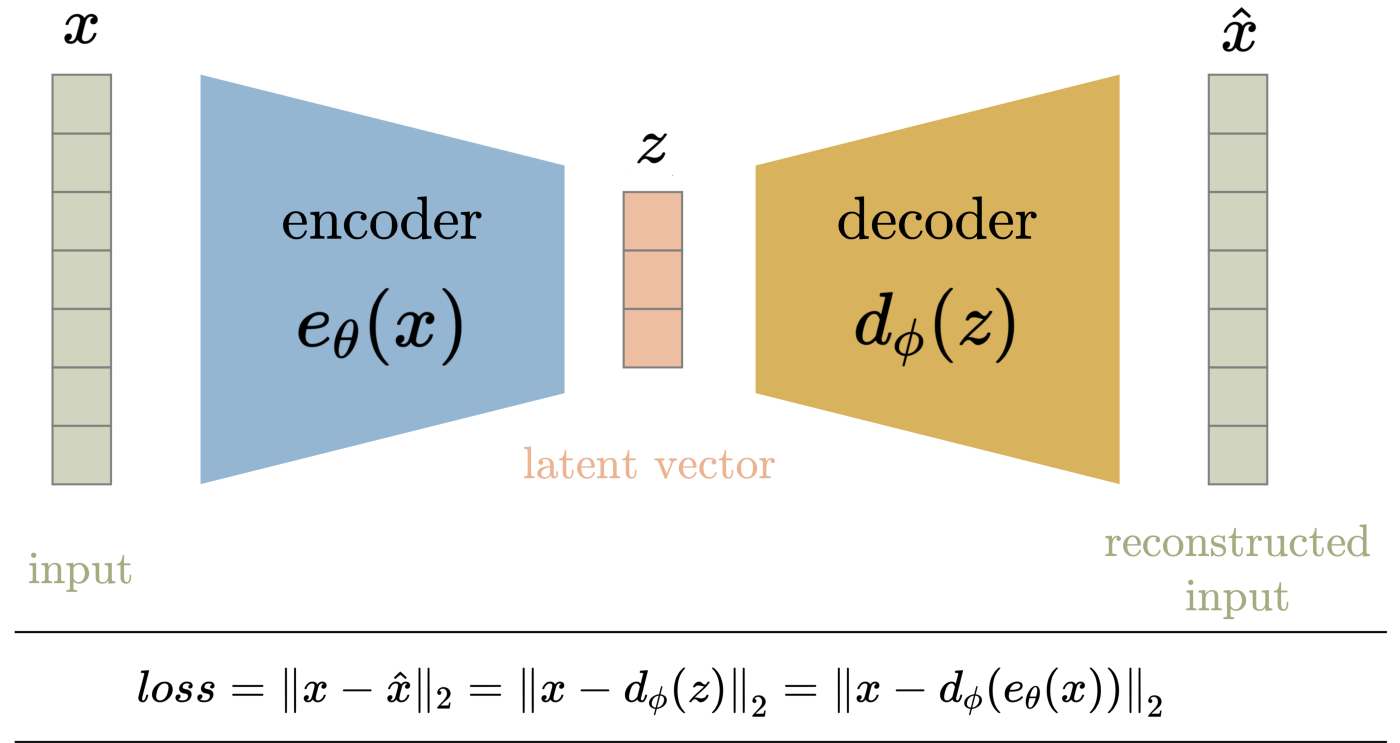
\includegraphics[width=0.70\textwidth]{background/ae.png}
  \end{center}
  \caption{AE diagram}
  \label{fig:ae}
\end{figure}

In other words, the encoder maps an image $x\in X$ into the latent space producing ${z=E_{\phi }(x)}$ with $z\in Z$; then $z$ is reconstructed by the decoder to bring it back to the original space ${x'=D_{\theta }(z)}$ with $x'\in X'$. Finally, $x'$ can be used as a label with any distance measure $d(x,x')$. Thus the loss to be minimized is computed as follows:

\begin{equation}
\label{eq:aeloss}
  L(\theta ,\phi ) = d(x_{i},D_{\theta }(E_{\phi }(x_{i})))
\end{equation}

\subsection{Variational AutoEncoder}

Variational AutoEncoders (VAEs) addresses the problem of \textit{sparse localization} of data points into the latent space thus providing a more powerful generative capability then AEs.

\begin{figure}[h]
  \begin{center}
    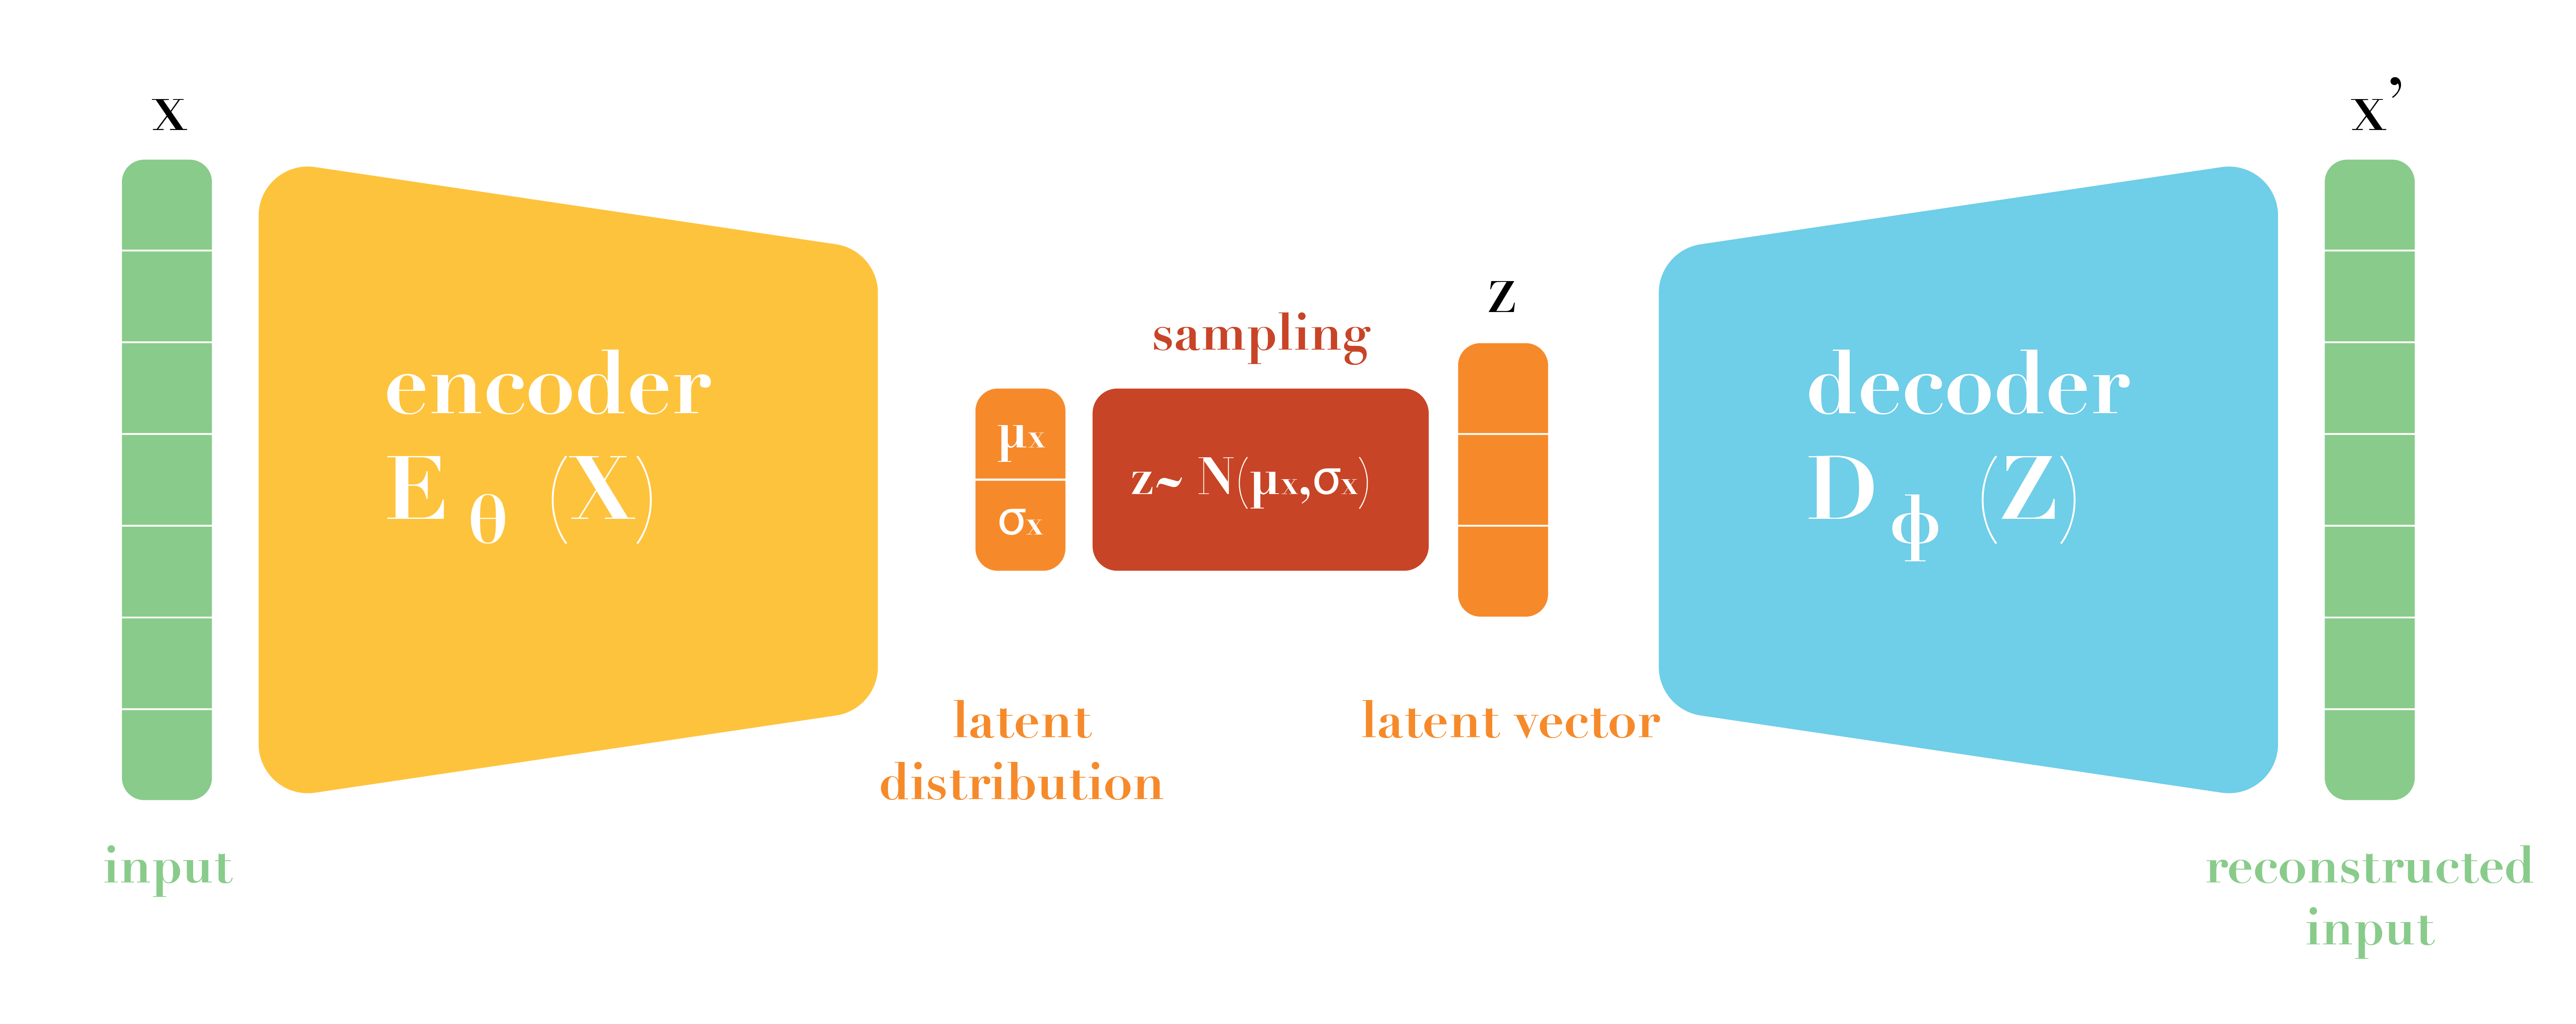
\includegraphics[width=0.80\textwidth]{background/vae.png}
  \end{center}
  \caption{VAE diagram}
  \label{fig:vae}
\end{figure}

As shown in Figure \ref{fig:vae} only a small change with respect to AEs is introduced, i.e. the encoder instead of mapping samples directly into the latent space it encodes a single input as a distribution (usually a normal distribution) over the latent space. Then the concrete latent vector $z$ is produced by sampling such distribution. 

Specifically, the encoder, starting from an image $x\in X$, produces the parameters ${[\mu_x, \sigma_x]=E_{\phi }(x)}$ such that $z$ is sampled from a normal distribution with such parameters $z \sim \mathcal{N}(\mu_x, \sigma_x)$. Consequently, the decoder brings it back to the original space ${x'=D_{\theta }(z)}$ with $x'\in X'$. Finally, $x'$ can be used as a label with any distance measure $d(x,x')$. Thus the loss to be minimized is computed as follows:

\begin{equation}
\label{eq:vaeloss}
  L(\theta ,\phi) = d(x_{i},D_{\theta }(E_{\phi }(x_{i}))) + KL[\mathcal{N} (\mu_x, \sigma_x),\mathcal{N}(0, 1)]
\end{equation}

where the first term is equivalent to the loss function in Equation \ref{eq:aeloss} and the KL term is the Kullback-Leibler divergence, which is a measure of how a probability distribution is different from another. The KL divergence acts as a regularization term by enforcing predicted distributions to be close to the normal distribution with mean 0 and standard deviation 1, giving to the latent space two main properties: continuity (close points in the latent space should be close also when decoded) and completeness (any point sampled from the latent space should always be meaningful once decoded). 

\section{DonkeyCar} \label{sec:donkeycar}

DonkeyCar, shown in Figure \ref{fig:donkey}, is an open source DIY platform providing software and hardware tools for the development of self-driving car algorithms. The basic car is a simple remote-controlled electric car that can be 3D printed or bought as a kit for an affordable price. The car can be customized with additional sensors as LIDARs and IMUs to provide more information about the surroundings of the car during driving.

\begin{wrapfigure}[19]{r}{0.5\textwidth}
  \begin{center}
    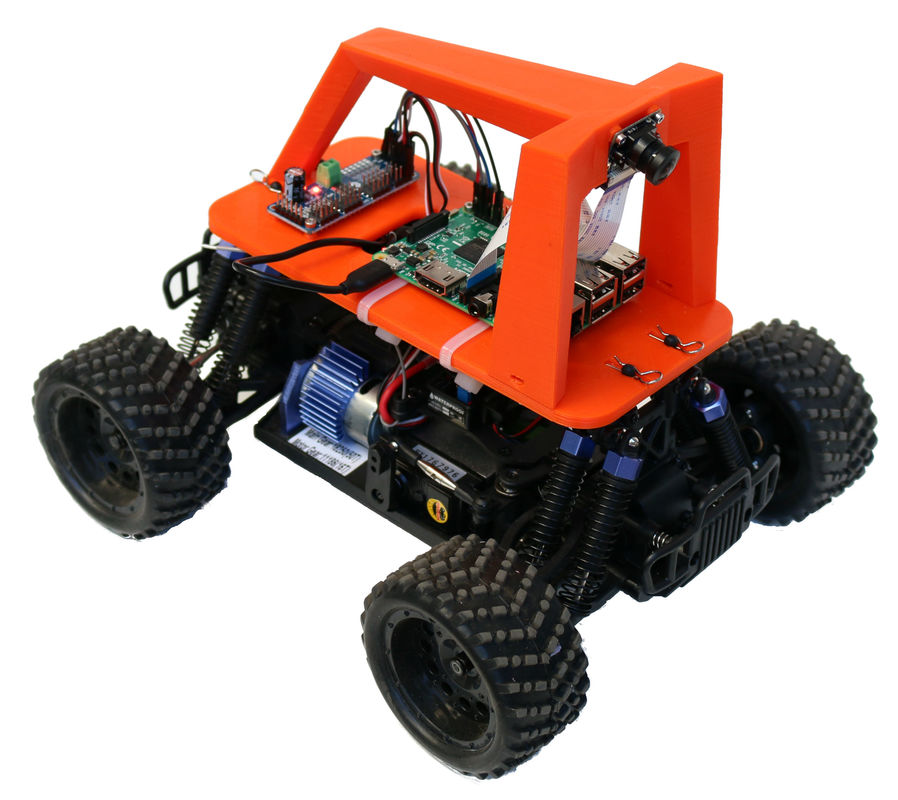
\includegraphics[width=0.5\textwidth]{background/donkey.jpeg}
  \end{center}
  \caption{Assembled DonkeyCar}
  \label{fig:donkey}
\end{wrapfigure}

In particular, the car used for the purposes of this thesis, is a basic DonkeyCar equipped with an 8-megapixel IMX219 sensor that features an 160 degree field of view. It is capable of capturing images with a resolution of 3280x2464 and video recording up to a resolution of 1080p at 30 frames per seconds. In order to process all the information coming from the camera, control the motors and run the self-driving car software, the car is equipped with an NVIDIA Jetson Nano micro-controller. The power comes from a LiPO battery of 11.1V and 2200mAh that runs the electric motor and the micro-controller. Additionally, to expand the operational life of the car, a power-bank can be added to exclusively power the micro-controller, while the LiPO battery is dedicated at powering the engine. 
A DonkeyCar can be remotely controlled either with a joystick or directly by the software.